%%%%%%%%%%%%%%%%%%%%%%%%%%%%%%%%%%%%%%%%%%%%%%%%%%%%%%%%%%%%%%%%
% 
% Sara Gergen                
% 351-53 
% Lab0
% 1/24/2023
% 
% 
%%%%%%%%%%%%%%%%%%%%%%%%%%%%%%%%%%%%%%%%%%%%%%%%%%%%%%%%%%%%%%%

\documentclass[12pt,a4paper]{article}

\usepackage[utf8]{inputenc}
\usepackage[greek,english]{babel}
\usepackage{alphabeta} 

\usepackage[pdftex]{graphicx}
\usepackage[top=1in, bottom=1in, left=1in, right=1in]{geometry}

\linespread{1.06}
\setlength{\parskip}{8pt plus2pt minus2pt}

\widowpenalty 10000
\clubpenalty 10000

\newcommand{\eat}[1]{}
\newcommand{\HRule}{\rule{\linewidth}{0.5mm}}

\usepackage[official]{eurosym}
\usepackage{enumitem}
\setlist{nolistsep,noitemsep}

\usepackage{cite}
\usepackage{lipsum}


\begin{document}

%===========================================================
\begin{titlepage}
\begin{center}

% Top 
\includegraphics[width=0.55\textwidth]{cut-logo-en}~\\[2cm]


% Title
\HRule \\[0.4cm]
{ \LARGE 
  \textbf{ECE 351 - Lab 0 }\\[0.4cm]
  \emph{Questions and Deliverables}\\[0.4cm]
}
\HRule \\[1.5cm]



% Author
{ \large
  Sara Gergen \\[0.1cm]
  January 17th\\[0.1cm]
  
}

\vfill

 
\end{center}
\end{titlepage}

%\begin{abstract}
%\lipsum[1-2]
%\addtocontents{toc}{\protect\thispagestyle{empty}}
%\end{abstract}

\newpage



%===========================================================

\addtocontents{toc}{\protect\thispagestyle{empty}}
\newpage
\setcounter{page}{1}

\begin{center}
    
\section{\LARGE Questions}

\end{center}

{\large
    \subsection{What did you do over last summer, or what are you planning to do this upcoming summer?}
}

\HRule \\[10]
   
    \textbf{This upcoming summer, I would like to learn many new skills; I plan to start more projects through a maker space called Gizmo. Another skill that I would like to broaden is my use of computers. I may install a Linux operating system on my computer to learn how a computer operates on a more basic level.
    Additionally, I would like to apply for possible internships to further my career. } 



{\large
    \subsection{What do you personally want to get out of this lab?}
}

\HRule \\[10]

    \textbf{I personally am excited to be able to comprehend Latex on a deeper level; the last time I attempted to learn it, I was frustrated and gave up since there was no purpose for me to use it. However, this class will allow me to discover a new way to format papers professionally. By messing around with the formatting and looking up the formatting on the provided cheat sheet, I was able to understand it better. I am also exhilarated to be able to learn python. I previously taught myself some python over break, and I am excited to not only test my knowledge, but also learn more about python. Here is a frog to show my excitement:}



\begin{center}

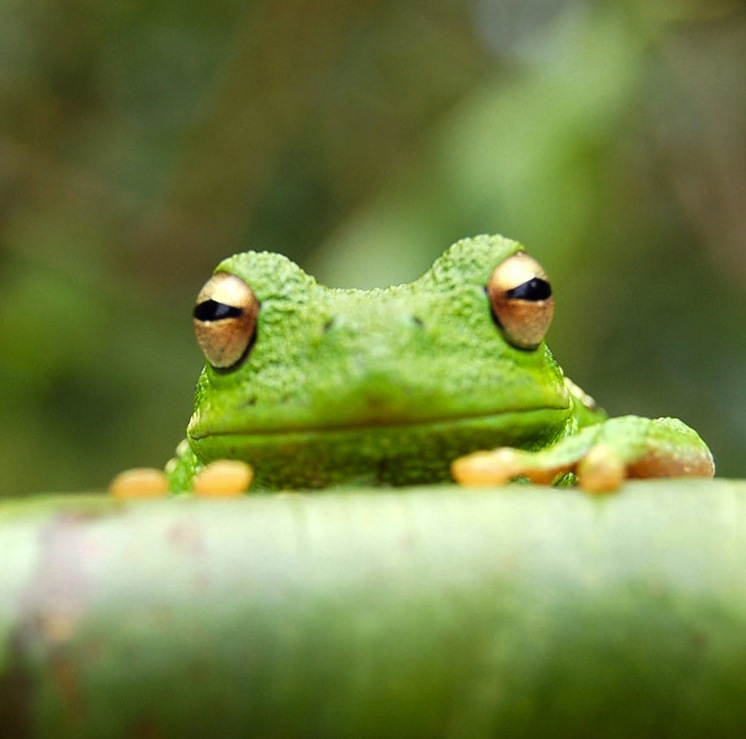
\includegraphics[width=0.3\textwidth]{frog.jpg}    

\end{center}

\end{document} 



